\chapter{Proposed Work}

\section{Problem Statement}
\emph{To develop a tool which can be used for automated social engineering attack on users of social networking sites using profile hijacking and man in the middle attack. Also test the tool via modified version of Turing test at basic conversation level}

\section{Passive Information Gathering Module}

\subsection{Social Networks}
A social networking service is an online service, platform, or site that focuses on building and reflecting of 
social networks or social relations among people, who, for example, share interests and/or activities and people 
with similar or somewhat similar interests, backgrounds and/or activities make their own communities.\\[0.5cm]
A social network service consists of a representation of each user (often a
profile), his/her social links, and a variety of additional services.\\[0.5cm]
Here are some statistics about Facebook (Alexa estimates, as of 20/04/2012):-
\begin{itemize}
\item{daily page views : ~8.4 billion}
\item{daily visitors : ~650 million}
\item{views per visitor : 12.9}
\item{site rank : 2nd}
\item{traffic fraction : 0.45\% ~1  in  220   of all web traffic }
\end{itemize}
\newpage
According to ComScore, Facebook has the largest number of Social Network User shares (up to end of November 2011)\cite{marketshare}\\

\begin{table}\large
\centering
\begin{tabular}{l | c | r}
Worldwide & Unique Visitors & Percentage\\
Facebook.com & 792,999 	& 55.1\%\\
Twitter.com & 167,903 & 11.7\%\\
LinkedIn.com & 94,823 & 6.6\%\\
Google Plus & 66,756 & 4.6\%\\
MySpace & 61,037 & 4.2\%\\
Others & 255,539 & 17.8\%\\
Total & 1,438,877 & 100\%\\
\end{tabular}
\end{table}
This shows that there is a lot of user generated information that is available to tap into. Facebook has its own API but we 
cannot use that to extract data about anyone. So we thought of writing a module which can do Web Scraping.
%Below is an example of how you will add references. short_paper_name is what you have specified in your ref.tex file
% so it will automatically do the [5] for you, or whatever number it is.

\subsection{Web Scraping}
Web scraping (also called web harvesting or web data extraction) is a computer software technique of extracting information from 
websites. Usually, such software programs simulate human exploration of the World Wide Web by either implementing low-level Hypertext 
Transfer Protocol (HTTP), or embedding a fully-fledged web browser, such as  Internet Explorer or Mozilla Firefox.\cite{wiki_scraping}

\subsection{Features}
This module will have the ability to scrape contents of facebook profile users page. It'll basically focus on the friends list of a user.
The data generated from this module will help in focusing on who are the victims friends, what are the statistics of them etc.\\[0.5cm]
Figure \ref{fig:myfriends} is a screenshot of a user and his friends list
\begin{figure}[htb]
\centering
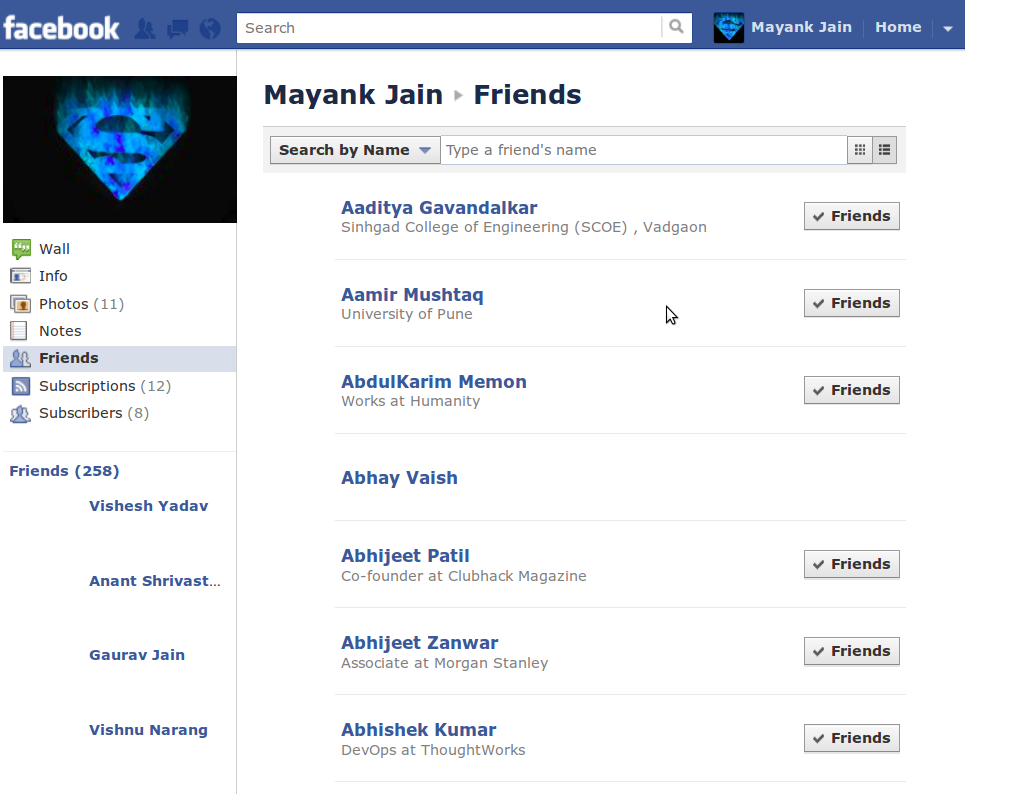
\includegraphics[scale=0.4]{project/diagrams/myfriends}
\caption{Friends List on Facebook}
\label{fig:myfriends} %see below of how to use it
\end{figure}

This module should be able to extract\\
\begin{itemize}
\item{Full Name}
\item{Gender : Male/Female/NA}
\item{username : Username/NA}
\item{Number of Friends : Total/NA}
\item{Unique UserID}
\end{itemize}

And in addition it should be able to extract each user's friends detail in a BFS Manner. And it can continue this as long as we want it to.

\section{Facebook Chat Attack Module}
\subsection{Extensible Messaging and Presence Protocol}
Extensible Messaging and Presence Protocol (XMPP) is an open-standard communications protocol for message-oriented middleware based on 
XML (Extensible Markup Language). The protocol was originally named Jabber, and was developed by the Jabber open-source community 
in 1999 for near-real-time, extensible instant messaging (IM), presence information, and contact list maintenance. Designed to 
be extensible, the protocol today also finds application in VoIP and file transfer signaling.\cite{wiki_xmpp}

Facebook uses XMPP (Extensible Messaging and Presence Protocol) for chatting.	

\newpage
\subsection{Attack as Example}
  Following is an example.\\
Lets say we have two marks (targets) Alice (Human) - aliceHuman and Bob
(Human) - bobHuman\\[0.5cm]
We make two profiles both run by bots. The highlight is bothbots hijack the
profilesof marks namely alice and bob.\\[0.5cm]
So aliceBots profile is similar to aliceHumans profile and bobBot’s profile
is simlar to bobBot’s profile. aliceBotsends a friend request to bobHuman.
bobBotsends a friend request to aliceHuman. So now, aliceHuman is a friend
of bobBot and bobHuman is a friend of aliceBot. Also, bobBot and aliceBot
can exchange information outside of facebook to each other.\\[0.5cm]
So now lets say, bobHuman and aliceHuman are online. Our bots start
the conversation. Whatever is being passed to one of the Bot by one human,
it is passed on to the other Bot and in turn passed on to the other human,
i.e. two humans are having conversation through two bots but they think
that they are talking to a human since the conversation sounds like a human
(which it is).\\[0.5cm]
After some amount of bonding between them our bots start modification
by using injecting questions inside the conversations\\[0.5cm]
\noindent
\textbf{AliceHuman - bobBot} : ”Hey how was the movie yesterday?”\\
\textbf{botBot - aliceBot} : ”Hey how was the movie yesterday?and hey btw whats
your fav color?”\\
\textbf{aliceBot - BobHuman} : ”Hey how was the movie yesterday? and hey btw
whats your fav color?”\\[0.5cm]
\textbf{BobHuman - aliceBot} : ”movie was great, and its blue btw, whats yours?”\\
\textbf{aliceBot - bobBot} : ”movie was great,you know my fav color is blue, what is yours?”\\
\textbf{bobBot - AliceHuman} : ”movie was great, you know my fav color is blue, what is yours?”\\[0.5cm]
\textbf{AliceHuman - bobBot} : ”mine is pink :)”\\
\textbf{botBot - aliceBot} : ”mine is pink :)”\\
\textbf{aliceBot - BobHuman} : ”mine is pink :)”\\[0.5cm]

Notice how the conversation has been altered to make it unclear that no
one asked each other about favorite color and yet both of them told us their
favorite color. We got hold of two marks information without raising suspicion.\\[0.5cm]


\begin{figure}[htb]
\centering
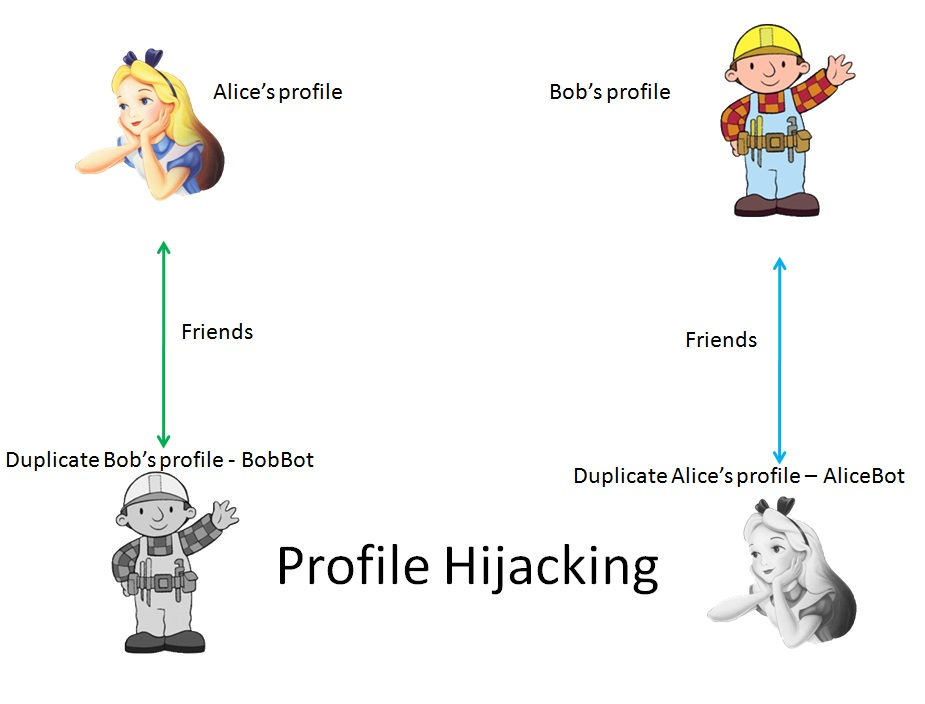
\includegraphics[scale=0.4]{project/diagrams/chatattack1}
\caption{Example of Profile Hijacking}
\label{fig:chatattack1} %see below of how to use it
\end{figure}

\begin{figure}
\centering
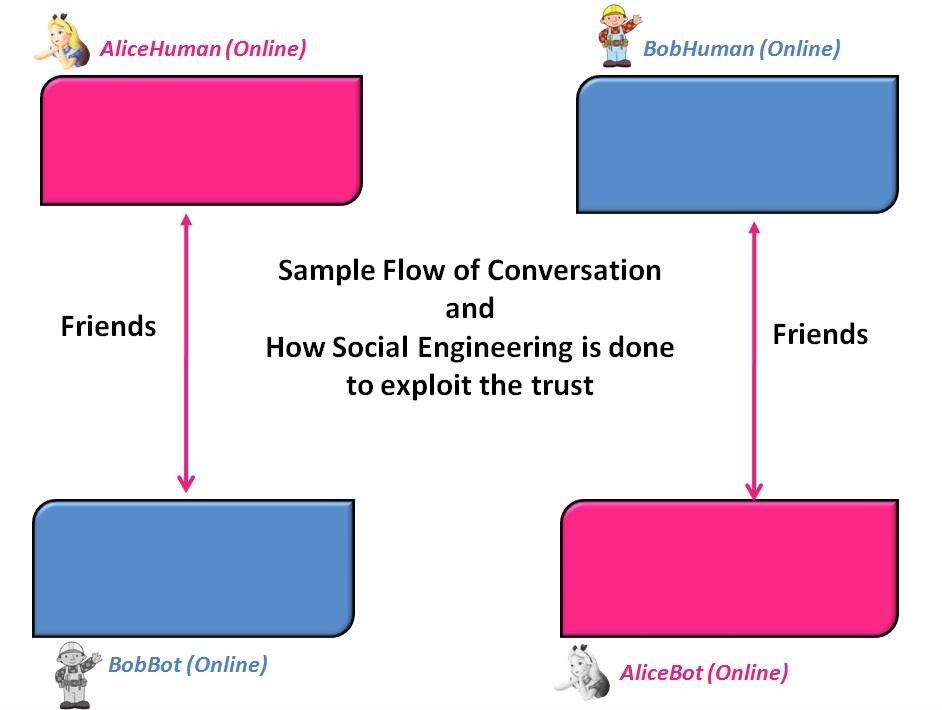
\includegraphics[scale=0.4]{project/diagrams/chatattack2}
\caption{Example of Conversation Modification - 1}
\label{fig:chatattack1} %see below of how to use it
\end{figure}

\begin{figure}
\centering
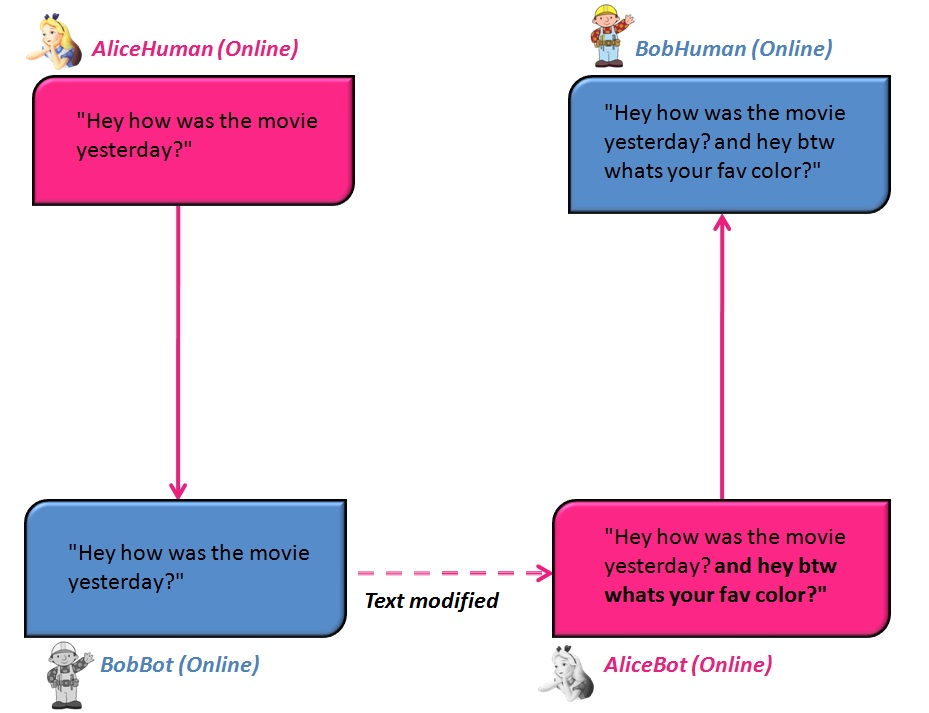
\includegraphics[scale=0.4]{project/diagrams/chatattack3}
\caption{Example of Conversation Modification - 2}
\label{fig:chatattack3} %see below of how to use it
\end{figure}

\begin{figure}
\centering
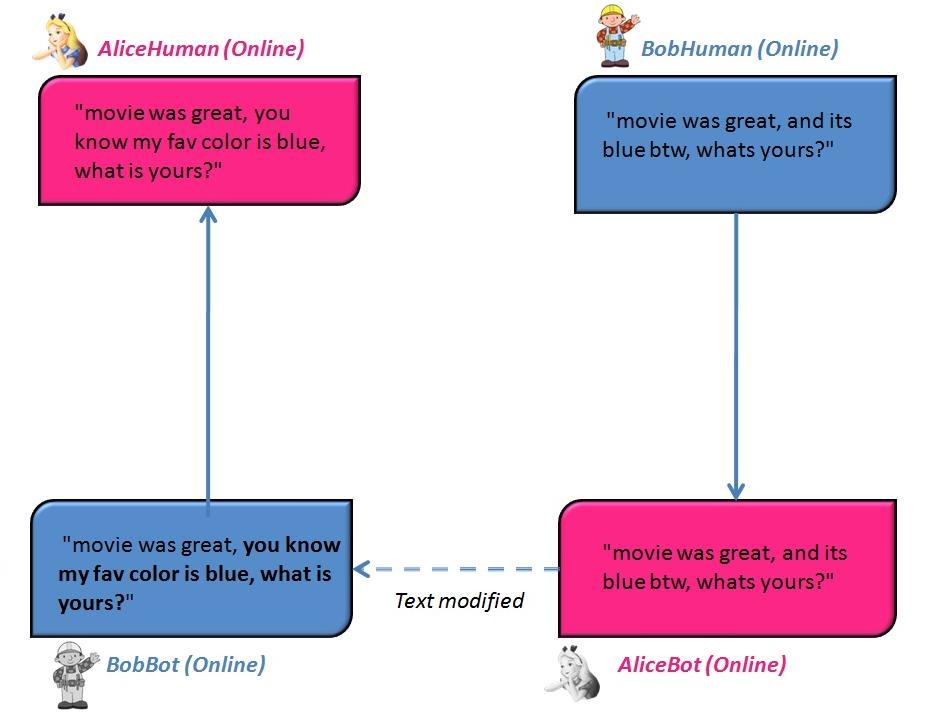
\includegraphics[scale=0.4]{project/diagrams/chatattack4}
\caption{Example of Conversation Modification - 3}
\label{fig:chatattack4} %see below of how to use it
\end{figure}

\begin{figure}
\centering
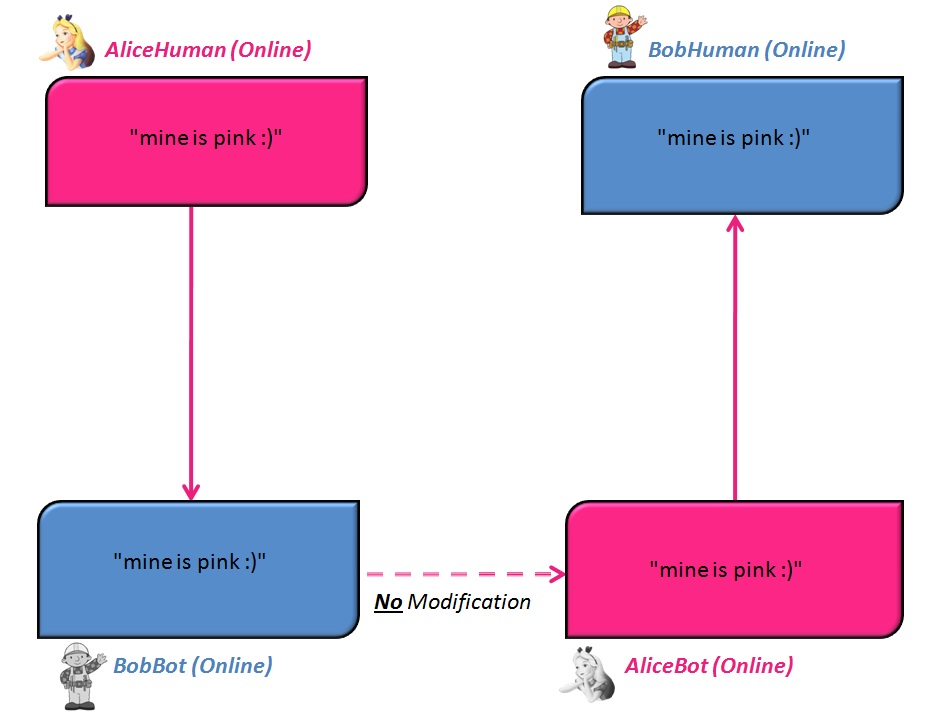
\includegraphics[scale=0.4]{project/diagrams/chatattack5}
\caption{Example of Conversation Modification - 4}
\label{fig:chatattack5} %see below of how to use it
\end{figure}

\newpage
\subsection{Constraints}
We will develop a POC (Proof of Concept) only. To modify the conversation we will use simple regex based parsing to match and substitute
it with matching strings. There will be no Artificial Inteligence or Machine Learning involved as that is out of scope at this level. Though 
it can be done and will make the modification more scalable and justified.